\section{Hypothesis Testing C.I.}
Motivation: Testing a specific $\betah_i$.

\nl We have $\betah = (X^TX)^{-1}Ty = [\betah_0, \dots, \betah_k]$. To pick off a specific $\betah_i$, we use the dot product.

\nl Let $e_i$ (standard basis vector), then $\displaystyle \betah_i = \underbrace{e_i \cdot \betah}_{\text{dot product}} = \underbrace{{e_i}^T \betah}_{\substack{\text{matrix} \\ \text{multiplication}}}$

\nl Note: $\E*{e_i \cdot \betah} = \E*{1 \cdot \betah_i} = \E*{\betah_i} = \beta_i$.
\\ Same with $\Var*{e_i \cdot \betah} = \Var*{\betah_i}$.

\nl So a test of the form
\begin{align*}
    H_0 &: \betah_i = (\beta_i)_0\\
    H_a &: \betah_i \neq (\beta_i)_0
\end{align*}
yields same old statistics.
$$Z = \frac{\betah_i - (\beta_i)_0}{\sqrt{\Var*{\beta_i}}} = \frac{\betah_i - (\beta_i)_0}{\sqrt{c_{i\,i}\sigma^2}} \qquad \text{with} \qquad [c_{i\,i}] = (X^TX)^{-1}$$
$$T = \frac{\betah_i - (\beta_i)_0}{S \sqrt{c_{i\,i}}} \qquad \text{with} \qquad n-(k+1) \text{ df.}$$

\example*
We fit
\begin{center}
    \begin{tabular}{|l|c|c|c|c|c|}
         \hline
         $x$ & -1 & 1 & 2 & 3\\
         \hline
         $y$ & 0.5 & -1 & -0.5 & 2\\
         \hline
    \end{tabular}
\end{center}
with $y = \beta_0 + \beta_1 x + \beta_2 x^2$ because it \say{looked} non-linear.
\begin{center}
    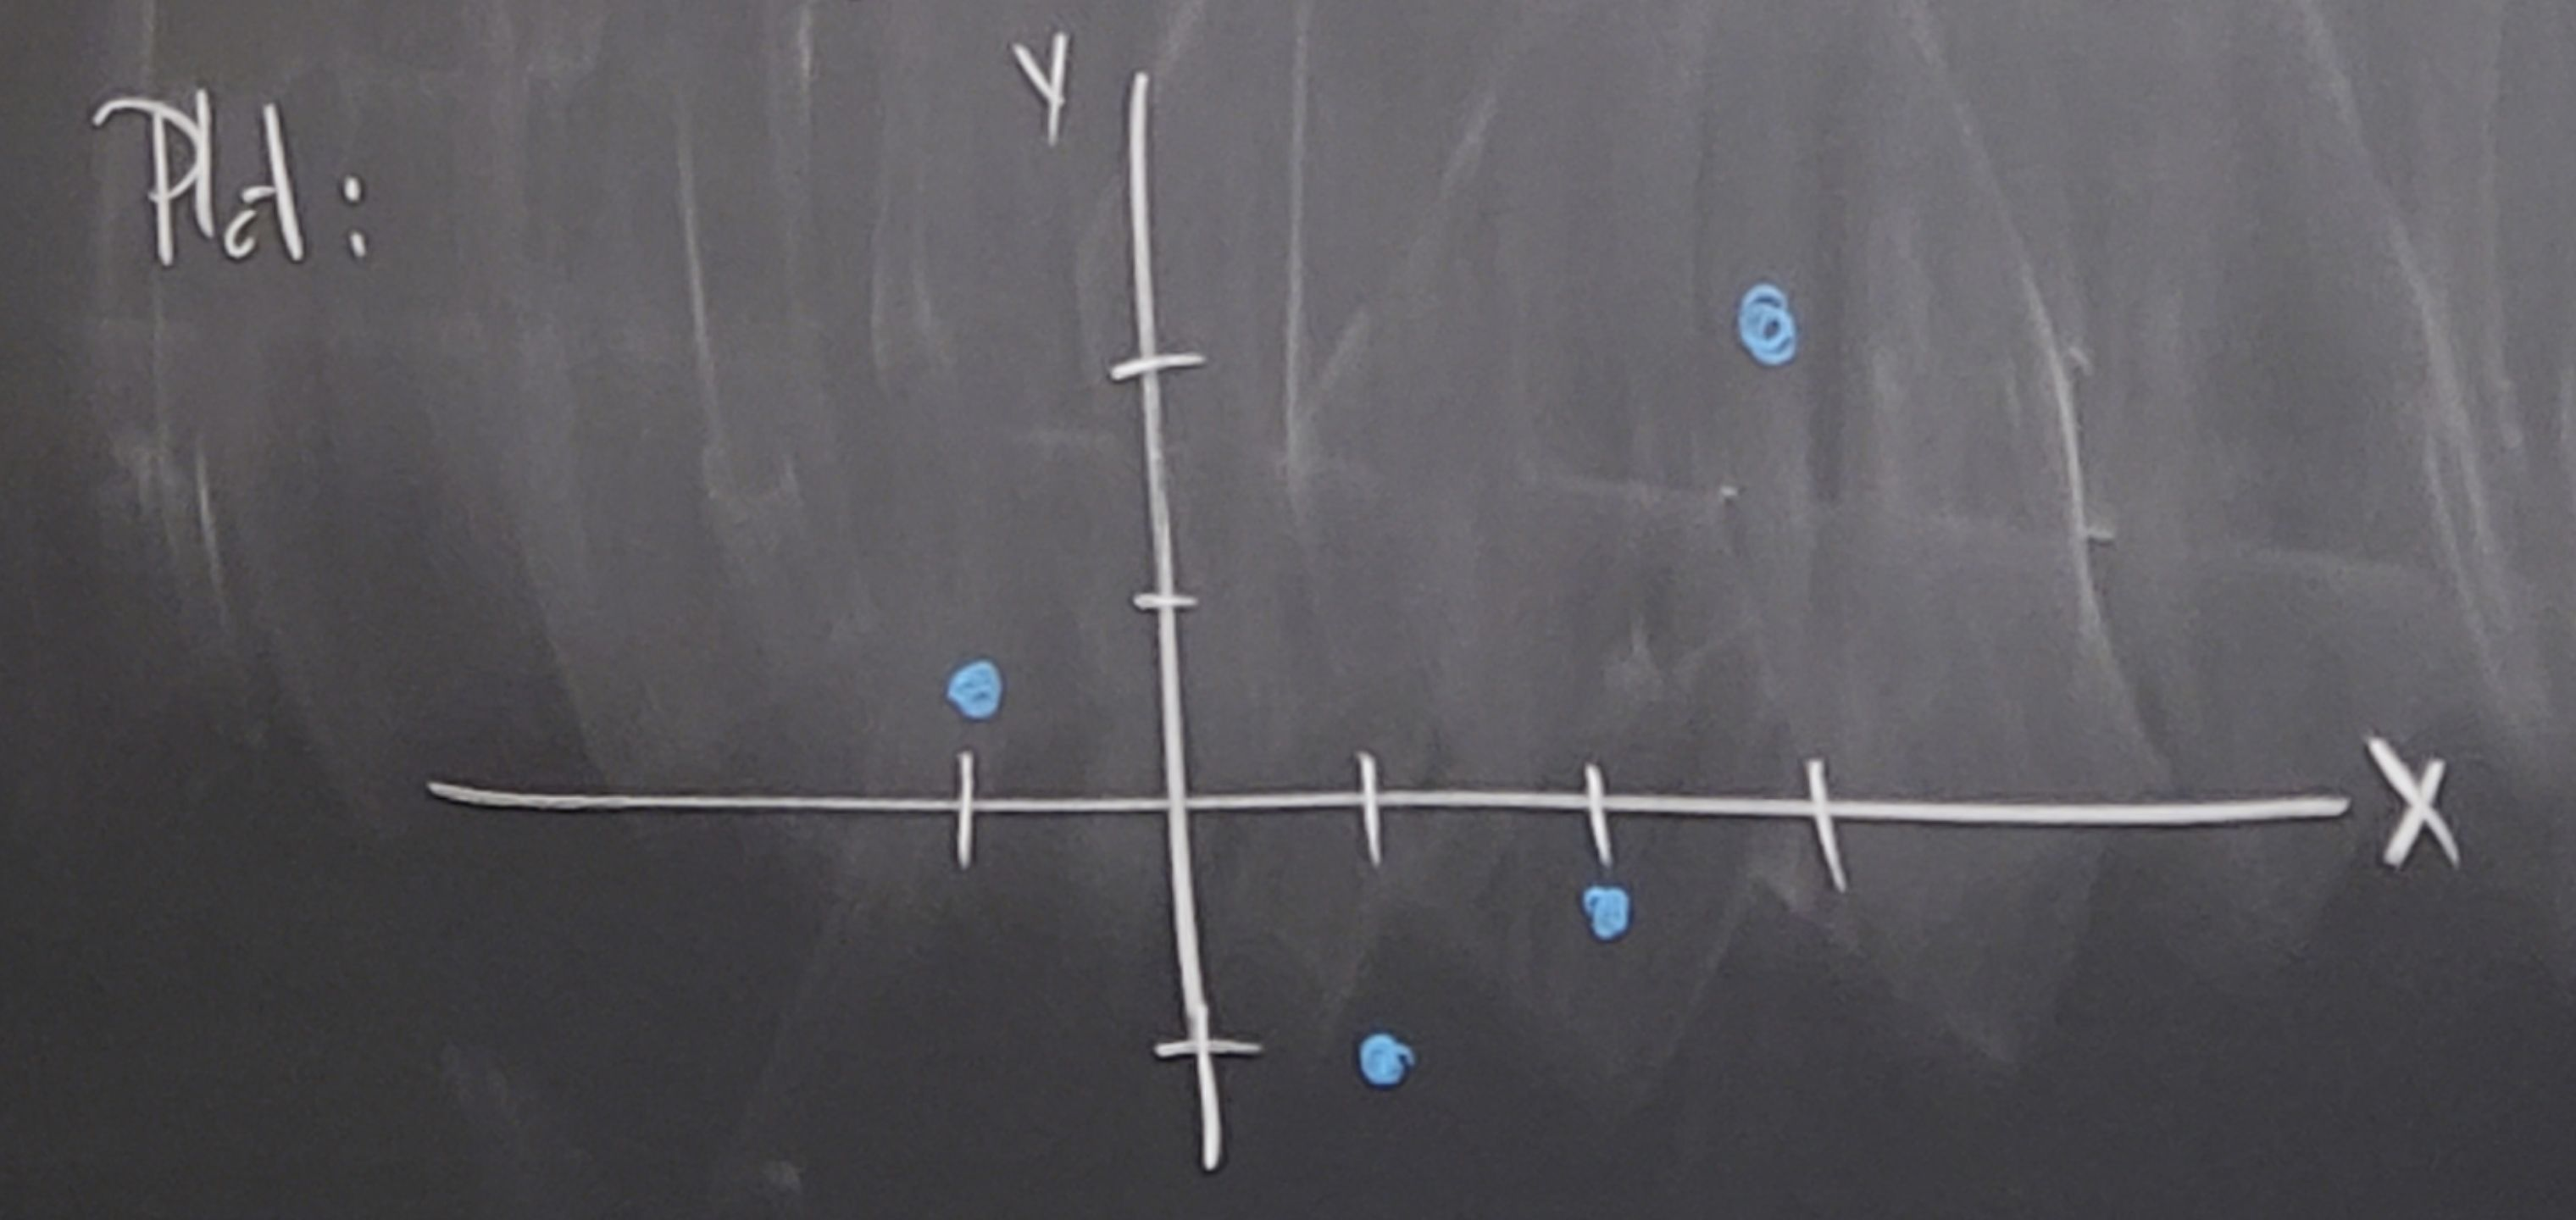
\includegraphics[height=2in]{11_10 plot.jpg}
\end{center}
Is there evidence that the data is in fact non-linear? That is, are we reasonably certain $\beta_{\alpha} \neq 0$.
\begin{align*}
    H_0 &: \beta_{\alpha} = 0\\
    H_a &: \beta_{\alpha} \neq 0
\end{align*}
We had
\begin{align*}
    \widehat{\beta} &= (\mathbf X^T \mathbf X )^{-1} \mathbf X^T y\\
    &= \begin{bmatrix}
        -41/44\\ -379/440 \\ 53/88
    \end{bmatrix}\\
    &= \vvec*{\betah_0}{\betah_1}{\betah_2}
\end{align*}
$e_3 = (0,0,1)$ and ${e_3}^T\betah = \dfrac{53}{80}$. We had
$$\mathbf X^T \mathbf X = \begin{bmatrix}
    4 & 5 & 15\\ 5 & 15 & 35 \\ 15 & 35 & 99
\end{bmatrix}$$
and $\det (\mathbf X^T \mathbf X) = 440$. Then
$$(\mathbf X^T \mathbf X)^{-1} = \over{440} \begin{bmatrix}
    260 & 30 & -50 \\
    30 & 171 & -65\\
    -50 & -65 & 35
\end{bmatrix}$$
With $\Var*{\betah_2} = c_{2\,2} \sigma^2 = \dfrac{35}{440}\sigma^2$. % was this beta2?

\nl For $\sigma^2$, we need $S^2 = \dfrac{\operatorname{SSE}}{n-2}$.
$$\operatorname{SSE} = y^Ty - \betah^T X^Ty = \frac{4791}{440}.$$
$$S^2 = \frac{\frac{4791}{440}}{n-2} = \frac{4791}{850} \approx 5.44432.$$
$$\Var*{\betah_2} \approx c_{2\,2} S^2 \cdots \sqrt{\Var*{\betah_2}} = 0.690201.$$
So
\begin{align*}
    T &= \frac{e_3 \cdot \betah - (\betah_2)_0}{\sqrt{\Var*{\betah_2}}}\\
    &= \frac{\frac{53}{88}-0}{0.690201}\\
    &= 0.872604
\end{align*}
$$\P{\abs{T} \geq 0.872604 \mid \df = 2} = 0.4748909.$$
\red{This sucks! It supports the null Hypothesis.}

\example* (Potency again)
\begin{center}
    \begin{tabular}{|l||c|c|c|c|c|c|c|c|c|c|c|c|}
         \hline
         $x$ & 30 & 30 & 30 & 50 & 50 & 50 & 70 & 70 & 70 & 90 & 90 &90 \\
         \hline
         $y$ & 38 & 43 & 29 & 32 & 26 & 33 & 19 & 24 & 23 & 14 & 19 & 21\\
         \hline
    \end{tabular}
\end{center}
I tried quadratic $y = \beta_0 + \beta_1x + \beta_2x^2$.
$$X = \begin{bmatrix}
    1 & x & x^2
\end{bmatrix}$$
$$(X^TX)^{-1} = \over{1.92 \times 10^6} \begin{bmatrix}
    1.092 \times 10^6 & -391200 & 3100\\
    -391200 & 14720 & -120\\
    3100 & -120 & 1
\end{bmatrix}$$
Note: $\Var*{\betah_2} = \over*{1.92 \times 10^6}\sigma^2 \approx \dfrac{S^2}{1920000}$.
$$\operatorname{SSE} = y^Ty + \betah^TX^Ty = 189.$$
$$S^2 = \frac{\operatorname{SSE}}{n-2} = \frac{\operatorname{SSE}}{10} = 18.9$$
$$\Var*{\betah_2} = 9.84775 \times 10^{-6}.$$
$$\sqrt{\Var*{\betah_2}} = 0.00313748$$
Testing
\begin{align*}
    H_0 &: \beta_2 = 0\\
    H_a &: \beta_2 \neq 0
\end{align*}
I computed $\betah_2 = \over*{1200}$.
$$t = \frac{\betah_2 - (\beta_2)_0}{\sqrt{\Var*{\betah_2}}} = 0.2656$$
With $\df = 10$, $\P{\abs{T} > 0.2656} = 0.79$, which is HUGE again. Hence it supports the null hypothesis.

\nl Of course, this is a math class and we love to generalive. We don't have to use a standard basis vector $e_i$. Let $\vec{a}$ be a constant vector $a = (a_0, \dots, a_k)$. Then
$$a^T\betah = a_0 \betah_0 + \dots + a_k \betah_k.$$
Note:
\begin{align*}
    \E*{a^T \betah} &= \sum{i=1}^k a_i \E*{\betah_i} \tag{by linearity}\\
    &= \sum{i=1}^k a_i \beta_i \tag{by unbiases estimators}\\
    &= a^T \beta
\end{align*}
for $\beta = (\beta_0, \dots, \beta_k)$. Also,
\begin{align*}
    \Var*{a^T \betah} &= \Var*{a_0 \betah_0 + \cdots + a_k \betah_k}\\
    &= \sum{i=1}^k \sum{j=1}^k \Cov (a_i \betah_i, a_j \betah_j)\\
    &= \sum{i=1}^k \sum{j=1}^k a_i a_j \underbrace{\Cov (\betah_i, \betah_j)}_{\substack{\text{These are } c_{i\,j} \sigma^2 \text{'s} \\ \text{from } (X^TX)^{-1}}}
\end{align*}
This entire double sum can be written as the matrix product
$$\Var*{a^T \betah} = a^T (X^TX)^{-1}a \cdot \sigma^2$$
% = 1xk, kxk, kx1
$$\implies Z = \frac{a^T \betah - \E{a^T \betah}}{\Var{a^T\betah}} = \frac{a^T \betah - a^T \beta}{\sigma \sqrt{a^T (X^TX)^{-1} a} }$$

\nl Given $H_0 : a^T \beta = (a^T \beta)_0$ versus some alternative, use
$$T = \frac{a^T \betah - (a^T \beta)_0}{S \sqrt{a^T (X^TX)^{-1}a}}$$
with $n-(k+1)$ degrees of freedom. 